\section{Related Works}
% % \subsection{Image-to-Image Transformation}
% \begin{frame}{Non-diffusion Methods}
%     \begin{itemize}
%         \item CNN
%         \item GAN
%     \end{itemize}
% \end{frame}


% \begin{frame}{Image-to-Image Transform}
%    % \begin{figure}
%    %     \centering
%    %     \includegraphics[width=0.9\linewidth]{img/im2im.png}
%    % \end{figure}
%    \begin{figure}
%        \centering
%        \includegraphics[width=0.9\linewidth]{img/I2IExample.png}
%    \end{figure}
% \end{frame}



\begin{frame}{Related Works: General Approach}
    \begin{figure}
        \centering
        \includegraphics[width=1\linewidth]{img/P0.png}
    \end{figure}
\end{frame}

% \begin{frame}{Related Works: U-Net based approach}
%     \begin{figure}
%         \centering
%         \includegraphics[width=1\linewidth]{img/removal-unet.png}
%         \caption{U-Net architecture for watermark removal \footnote{Fu, Lijun, et al. "An improved u-net for watermark removal." Electronics 11.22 (2022): 3760.}}
%     \end{figure}
% \end{frame}

\begin{frame}{Related Works: GAN-based Approach}
   \begin{figure}
       \centering
       \includegraphics[width=0.45\linewidth]{img/r2architechture2.png}
       \caption{The GAN architecture for watermark removal \footnote{\scriptsize Cao, Zhiyi, et al. "Generative adversarial networks model for visible watermark removal." IET Image Processing 13.10 (2019): 1783-1789.}}
   \end{figure}
\end{frame}

\begin{frame}{Related Works: SWCNN}
    \begin{figure}
        \centering
        \includegraphics[width=0.8\linewidth]{img/swcnn.png}
        \caption{SWCNN architecture \footnote{Tian, Chunwei, et al. "A self-supervised CNN for image watermark removal." IEEE Transactions on Circuits and Systems for Video Technology (2024).}}
    \end{figure}
\end{frame}


% \begin{frame}{Diffusion Models}
%     \begin{figure}
%         \centering
%         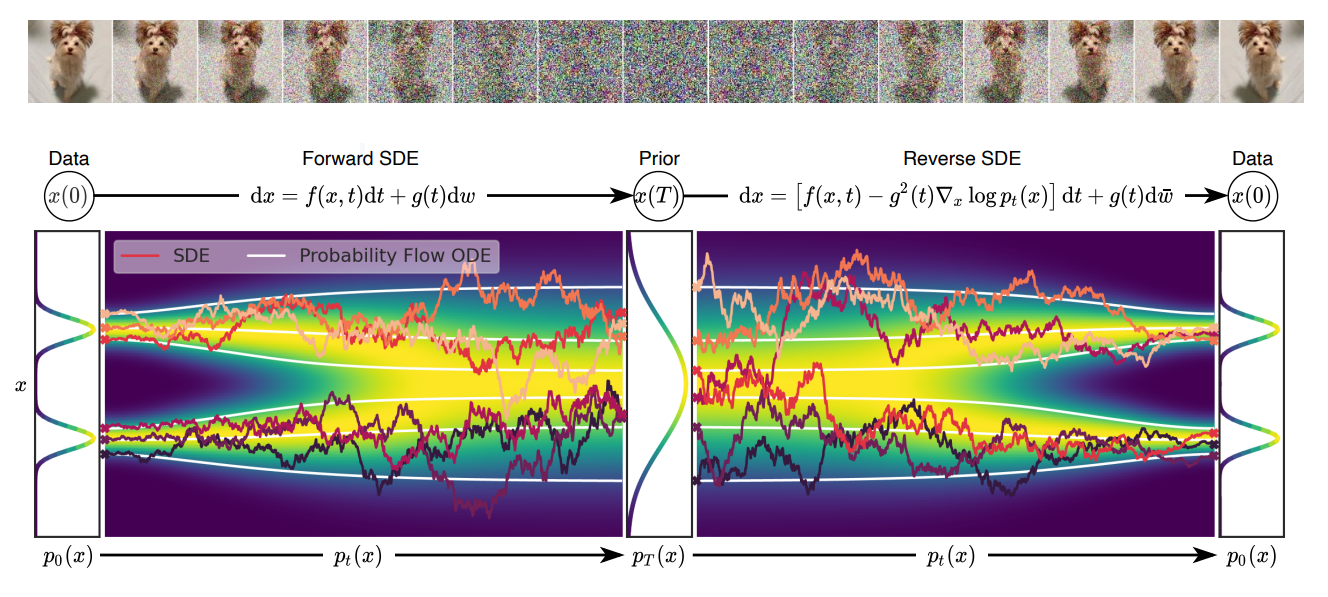
\includegraphics[width=1\linewidth]{diffusion.png}
%         \caption{Diffusion models as two Markov chains \footnote{Song, Y., \& Ermon, S. (2019). Generative modeling by estimating gradients of the data distribution. Advances in neural information processing systems, 32.}}  
%         \label{fig:enter-label}
%     \end{figure}
% \end{frame}
